 % -*- root: ../medieninformatik-arbeit.tex -*-
\documentclass[../medieninformatik-arbeit.tex]{subfiles}
\begin{document}
	

\section{Related Work}
\label{ch:related}
In this chapter projects related to product configurators and activity
sculptures will be presented. Each work presents a unique solution to the addressed problem, 
the approach each author took will be discussed and the adaptation of useful knowledge to this
work will be explored. To conclude the chapter an overview of available vendor
API for data import will be presented. 

\subsection{Web-based Interactive Product Visualization}
This work has a particular interest in product configurators that make use of 3D
computer graphics to visualize the product. The majority of modern web
configurators are image based and make use of well designed backgrounds to place the
product in well perceived environment. For example the UNU electric scooter
configurator puts the scooter on a street background that
changes as the user moves to the next step of the configuration (fig.\ref{fig:unu-config}). 
Other systems may opt for a more minimalistic look, and will try to isolate the
product and place it in a white background as seen on
figure \ref{fig:timbuk2-config}. 
Although this might work for some products the user still misses some of the benefits of
interacting with a spatial representation the products\cite{vande2009analyzing}.
One of the main challenges of developing  configurator systems is the modeling
of the relation between the product configuration and its visual representation
and the correct rendering of the visual representation in real
time\cite{feliceinteractive}. The advantage of a 3D visualization system
over an image based one, is that the different configurations can be generated on
the fly instead of using complex logic systems to retrieve the correct image
combination from an image database. On the following section, three product
configurators will be presented that use novel 3D visualization technologies to
offer users a robust interactive tools for designing unique products.

\begin{figure}[h]
\captionsetup{width=0.4\textwidth}
\centering
\begin{minipage}{.45\textwidth}
\centering
  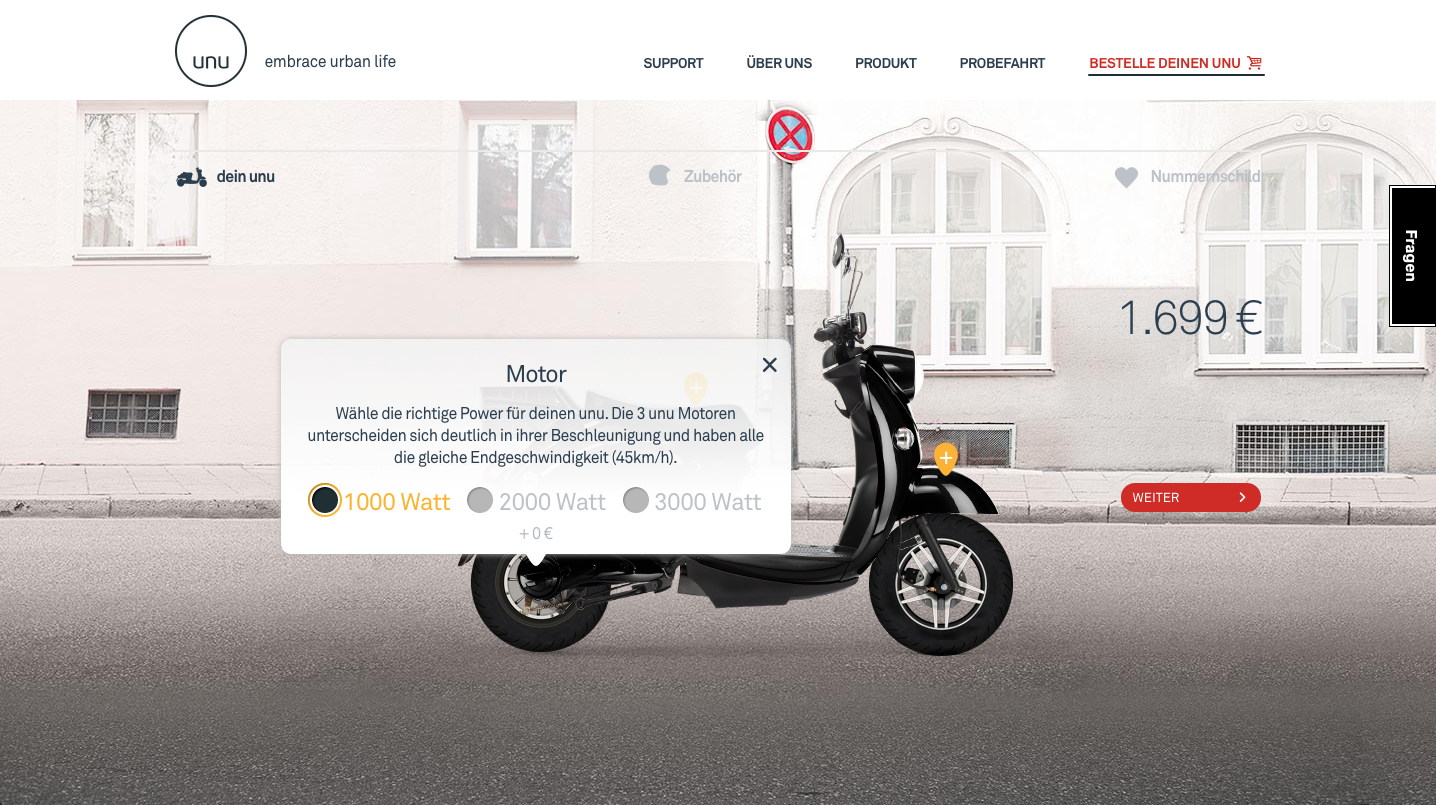
\includegraphics[width=\linewidth]{RelatedWork/img/unu-config}
  \caption{\protect UNU electric scooter web configurator\cite{unu:2015:Online}}
\label{fig:unu-config}
\end{minipage}
\begin{minipage}{.45\textwidth}
\centering
  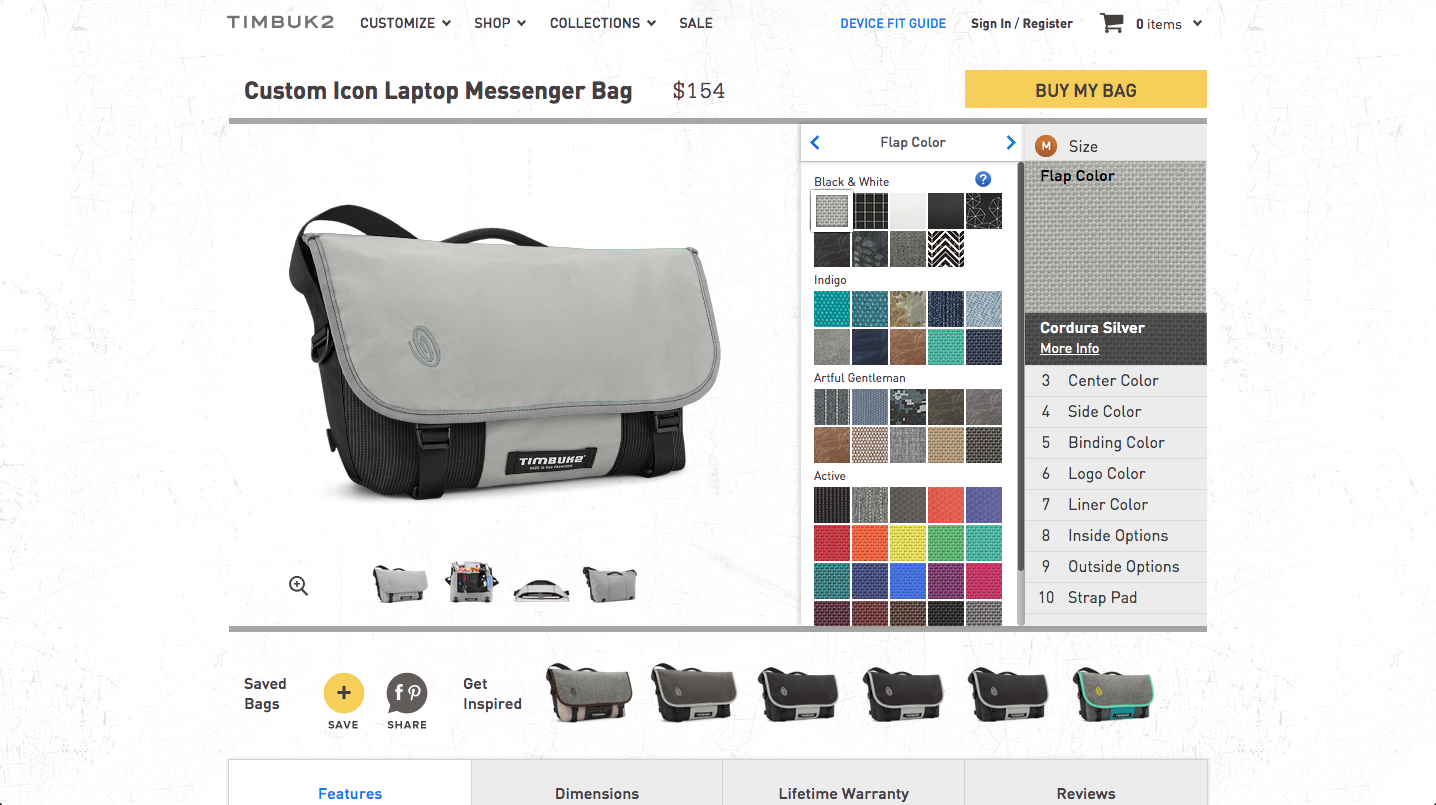
\includegraphics[width=\linewidth]{RelatedWork/img/timbuk2-config}
  \caption{\protect Timbuk2 bag web configurator\cite{timbuk2:2015:Online}}
\label{fig:timbuk2-config}
\end{minipage}
\end{figure}

\subsubsection{Gates 3D Configurator}
As part of an action-research project from Living
Lab\cite{livinglabs:2015:Online} Rolland et al.\cite{rolland2012commerce}
developed a gate configurator for the French company Groupe Maine's gates. The
objective of the authors was to showcase the possibilities of 3D Web
technologies in e-commerce applications. The developed tool was build with the
Unitiy3D\cite{unity3d:2015:Online} game engine, a flexible tool principally
build for game development but it has proved to be also useful for architectural
visualization and graphic intense web applications. After a user has logged in
to the configurator, the platform allows customers to select from a variety of
gate styles visualized as 3D models placed on the right side controls (see fig.\ref{fig:gates-config}). The user has also the option of setting the environment in which the gate is being placed (left side controls). This can happen by either selecting a predefined environment of by uploading a picture of the user's home or place where the gate shall be installed later. Customers can position the gates in the uploaded photograph by operating dedicated slider controls. The main advantage of allowing customers to upload their own images is that this allows them to have a better idea of how the selected gates will look in the final environment making them feel more comfortable about their decision. The authors state that they preferred the superimposition of a custom image rather than letting the user customize the environment with threes or buildings to make it look as close as possible because of the possible frame rate drop produced of handling many models and generating and because it is quite rare that somebody has a 3D model of his home. 

One of the main aspects of the gates configurator in respect to the research purposes the authors had, was that of developing a tool that improved the visualization of products with the end of encouraging the purchasing of the product in an on-line medium. To validate the design ideas behind the gate configurator and analyze the impact it had on customers, the authors performed an empirical evaluation. The results of the 27 evaluated participants showed that the manipulation of objects in 3D space seem naturally and was also confirmed to be important to the participants to have this option. This shows that having a realistic view of the product improves the chances of sale.

\begin{figure}[hb]
\begin{center}
  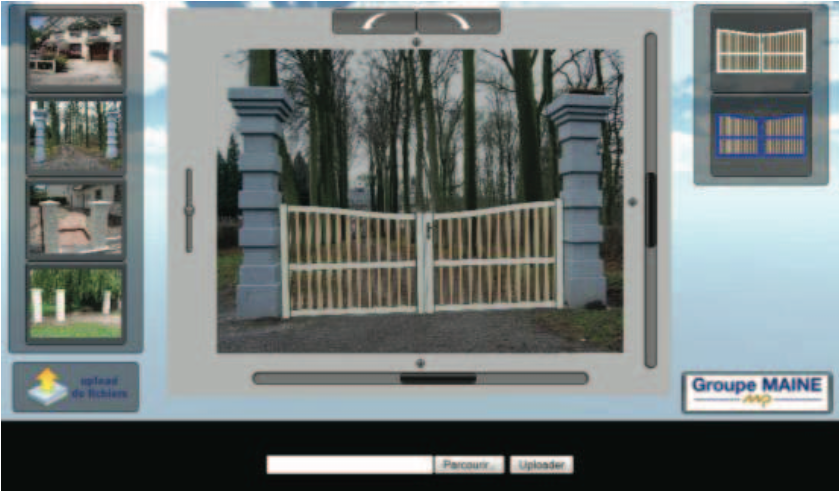
\includegraphics[width=0.7\textwidth]{RelatedWork/img/gates-config}
  \caption{Groupe Maine's gates configurator\cite{rolland2012commerce} }
\label{fig:gates-config}
\end{center}
\end{figure}

The gates configurator is a great example of how companies can make use of 3D visualization technologies to present their product to customers in a more convincing way. The authors of made a great choice of working with the Unity3D game engine as it allows them to port to other platforms as well, in this way developed software tools could be very easily ported to other mobile platforms like tablets or smartphones with bigger screens without the need of starting from scratch. This technology also offers desktop like frame rate performance in the web. The configurator has not many configuration possibilities which makes it easier for customers to understand but it excels at providing different visualization environments which in this case takes advantage of navigating in 3D space. One key statement of the authors was that tools like the configurator promote customer's participation in the developing of products. It was a shame there is no actual configurator in the Groupe Main's webpage for testing and it is unknown if the configurator was ever implemented in their website. The authors of the gates configurate see a great potential of 3D visualization technologies in fields such as e-learning, simulation and education.

\subsubsection{The MakerVis Fabrication Tool}
The MakerVis fabrication software is, in the words of its creators: \textit{``a prototype tool that integrates the entire process of creating physical visualizations, from data filtering to physical fabrication''}\cite{swaminathan2014supporting}. If somebody attempts to visualize their information they will have to use a wide range of tools to achieve this. This is cumbersome and impractical as it requires a great amount of effort and in general it is a very conflict prone way of working with data. This motivated Swaminathan et. al to develop MakerVis as an attempt to offer a platform that unifies the needed tools to extract data, filter it and visualize it. Although the focus of the MakerVis is not the implementation of a complex tool but more the exploration of the different challenges encountered in the process of visualization.

The work-flow provided by MakerVis is composed of six steps all displayed in the user interface seen on figure \ref{fig:makervis-config}. First users need to upload a CSV file containing the data to visualize. After that users can select between several visualization styles. Once a visualization is selected the data the user can begin mapping the data to the visualization by selecting data variables. Further on users can manipulate the visualization's geometry through an array of sliders and controls. In order to setup fabrication parameters and selecting the machine users can make use of the lower right section where the visualization is deconstructed layer by layer. Finally the STL file of the model can be exported for fabrication. A helpful functionality the authors implemented was the specification of printing materials through a JSON file.  It is worth mentioning that MakerVis does not provide true 3D visualizations. The produced designs are indeed physical objects but the final result is a pseudo 3D visualization. In order to achieve this the authors use principally 2D fabrication methods employing laser cutting and CNC machines, only basic 3D printing support is provided. The visualizations users can choose from are more directed to traditional charts and bar graphs and not so much geared towards more artistic representations. Due to the modular engineering of tool, the visualizations can be expanded. The available tools for data manipulation is also limited and advanced manipulation should be better performed in an external tool. MakerVis was build with modern web technologies based on the JavaScript programming language like Node.js\cite{joyent2015node}, Three.js\cite{cabello2010three}, D3.js\cite{bostock2015d3js} and jQuery\cite{jqf2015jquery}. As some of this technologies were also used in the Activity Sculpture Configurator they will be explained in depth in Chapter \ref{ch:configurator}. 

Although the authors conducted a relative small user study, the results provided valuable information about what areas can be further improved. The user study showed that users wanted more detailed control about the decorative aspects of visualization. Providing tools for personalize text labels and scales increases would allow users to further customize their visualization. Another challenge encountered was that of material representation. It was difficult for users to decide on which materials to use and expressed the desire to physically interact with the available materials. Also the correct scale representation of the object was estimated wrongly by most users. The need of the ability to save and load visualizations was also expressed to be needed. This findings might sound as failures but they only make clear the limitations of the screen as a medium to transmit haptic properties of materials and that unifying every tool needed for data visualization in a tool is an immense challenge.

\begin{figure}[h]
\begin{center}
  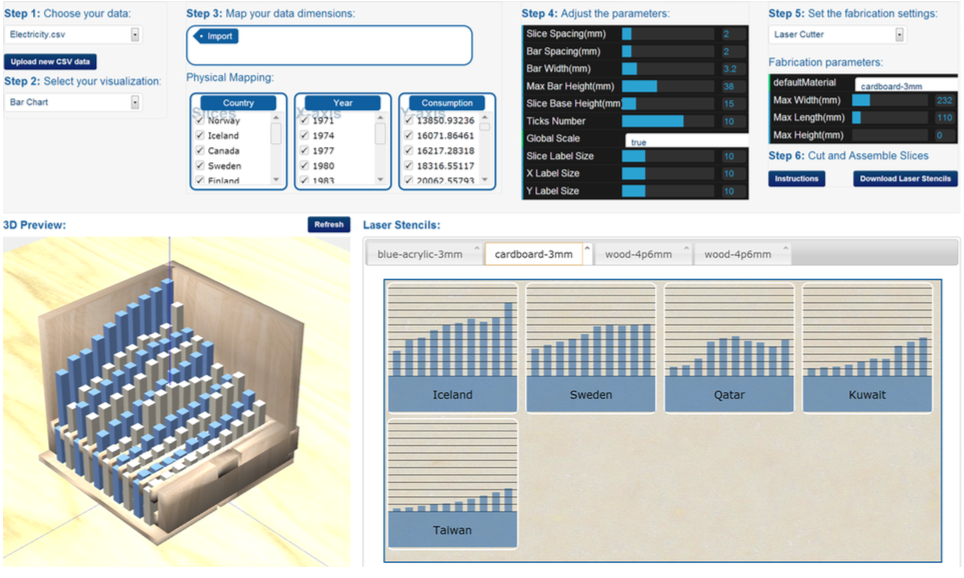
\includegraphics[width=0.7\textwidth]{RelatedWork/img/MakerVis}
  \caption{The MakerVis fabrication tool\cite{swaminathan2014supporting} }
\label{fig:makervis-config}
\end{center}
\end{figure}

The MakerVis fabrication tool approximates closely the aim of the work discussed in this thesis. This work shares the same mission of building a tool were the whole process of visualizing a 3D object is contained. The MakerVis focuses more on data manipulation and fabrication as it basically dedicates two thirds of the whole screen to data filtering and fabrication parameters. None the less the interaction concepts and design layout served as a reference point for the activity sculpture configurator. 

\subsubsection{Twikit}
The 3D printing market is a fast growing market estimated to reach US\$16.2 billion dollars in value by 2018\cite{canalys2014trends}. Many see the potential to offer services to facilitate the design and production of 3D printing goods. An interesting example is 
Twikit\cite{twikit2015tech} a company located in Belgium that offers innovative software, fabrication and shipping solutions for brands and retailers looking to easily implement product customization to their product portfolio. The Twikit website\cite{twikit2015tech} states that their goal is to ``allow end-to-end 3D product customization, in the easiest way possible'' and they see 3D product customization as ``key in the future of products and experiences''.

The range of services the belgian company offers covers every step in the development of a 3D configurable product. If needed Twikit is can aid brands in the development of their 3D product through collaboration with existing design teams. On the software side, Twikit offers a complex engine for 3D visualization, customization and fabrication called Twikbot. This engine allows companies to integrate customization tools into their current e-shop or application. Due to the modular nature of the engine, retailers can choose what kind of interface controls they need for the customization process and integrate them with the assurance that the design specifications and constraints will be met. The Twikbot also offers material configuration functionality for a variety of 3D printing techniques. Another integral component of the Twikbot is its Content-Management-System (CMS). The Twikbot CMS is a backend tool that manages and tracks currently configured and sold products and through an API cloud-based service it links to logistics and 3D print fulfillment providers. 

The Twikit website showcases several study cases from small and large businesses that have integrated their software to sell appealing customizable products. As much as it would be interesting to know how Twikit performs in all areas of their services, for the purposes of this thesis, only the configurators showcased will be evaluated. One interesting case study in the website is the 3D Trophy Factory\cite{twikit2015tech} which is owned and run by the same Twikit people. This e-shop sells a variety of trophy models were the text can be customized (see figure \ref{fig:trophy-config}). It is a very simple configurator that allows customers to interact the trophy in 3D space through click and drag. Depending on the model customers can input up to three different text lines. The configurator offers the possibility to save and load configured trophies. If users have a custom 3D model they would like to print as a trophy, the e-shop supports uploading 3D model files. In some designs users can also change some text properties like randomize the positioning. 

\begin{figure}[h]
\captionsetup{width=0.4\textwidth}
\centering
\begin{minipage}{.45\textwidth}
\centering
  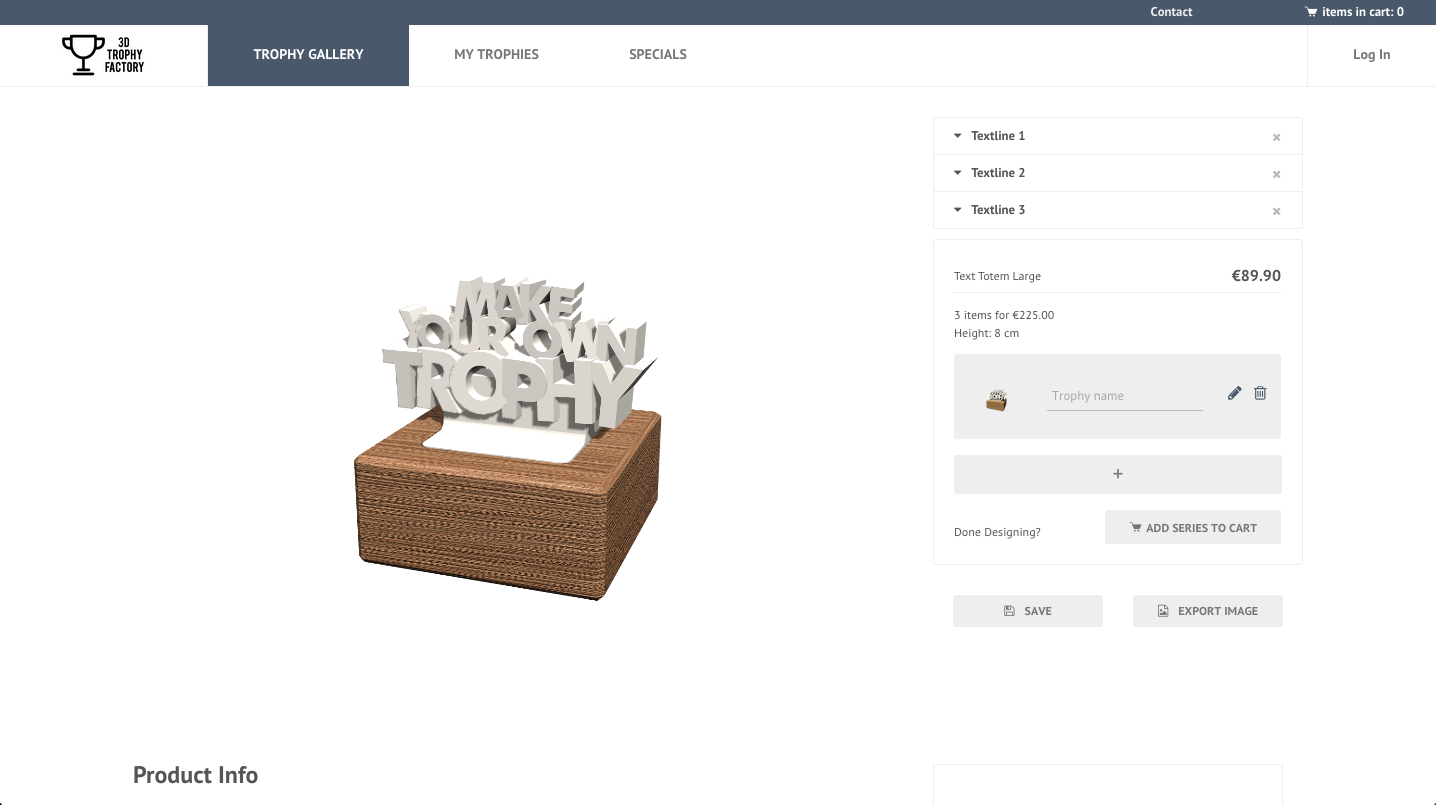
\includegraphics[width=\linewidth]{RelatedWork/img/trophy-config}
  \caption{\protect Twikit powered 3D Trophy Factory web configurator\cite{trophy2015factory}}
\label{fig:trophy-config}
\end{minipage}
\begin{minipage}{.45\textwidth}
\centering
  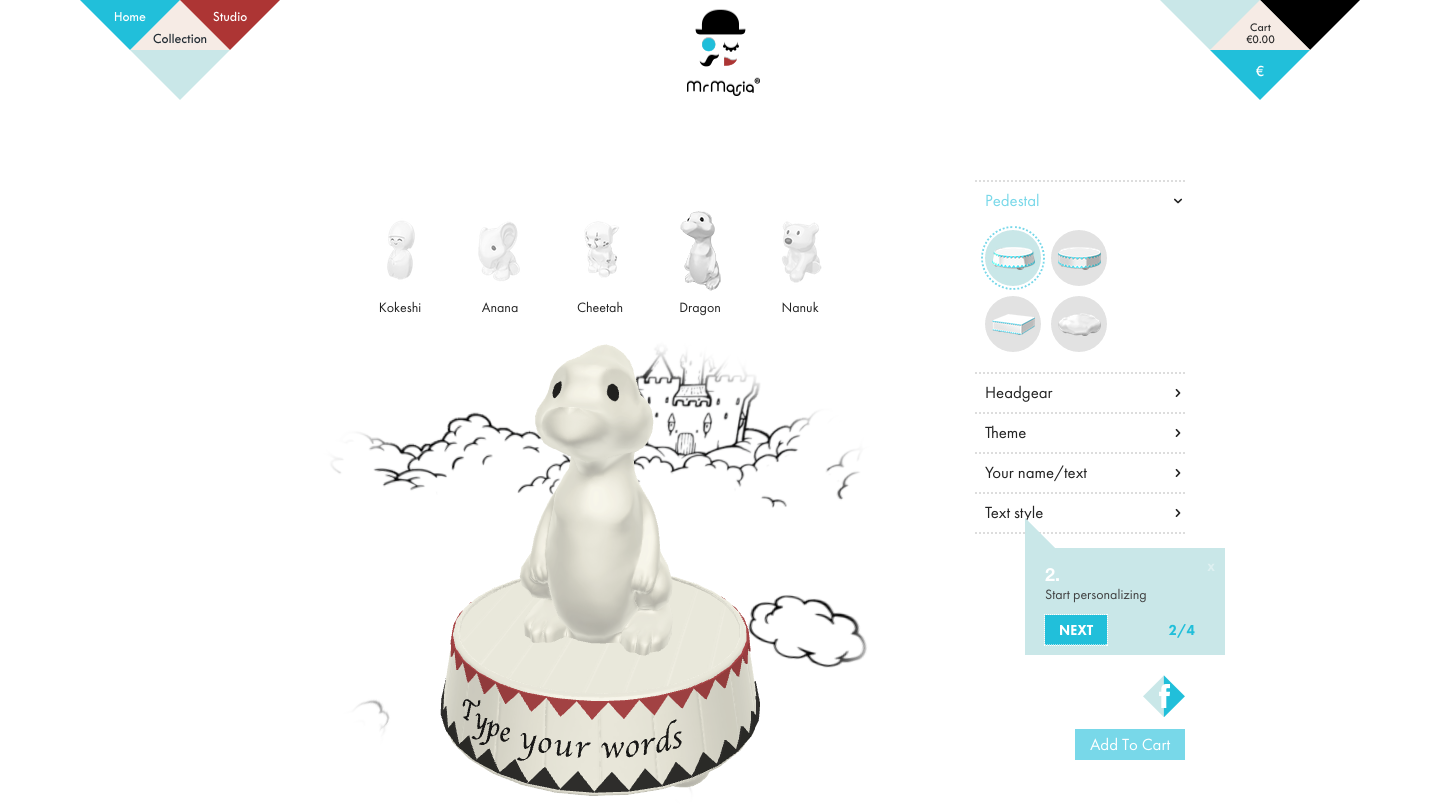
\includegraphics[width=\linewidth]{RelatedWork/img/mrmaria-config}
  \caption{\protect Twikit powered MrMaria Studio lamp web configurator\cite{mrmaria2015studio}} 
\label{fig:mmaria-config}
\end{minipage}
\end{figure}

The next Twitkit case study shows that the technology offered by Twickit can be easily used to enable brands no matter how big or small to start offering customizable products. Amsterdam based design studio Mr Maria\cite{mrmaria2015studio} added a customizable toy lamp to their product line. The lamp configurator showcases the brand identity of the studio and allows customers to customize their lamp in a playful way. The lamp is composed by a model of an animal and a pedestal were a text is placed. Users can choose different animals to place over the pedestal and further customize it by adding different accessories like hats, different pedestal designs with different color themes and a text field for adding a custom text (see figure \ref{fig:mmaria-config}. The lamp is placed in a cartoon style background which can be changed to a dark view where the lamp glows simulating to be turned on.  

The 3D Trophy Factory and the Mr Maria lamp configurator were both very appealing and fun to work with. Twikit does not say much about the technologies used in the framework but a view into both e-shop's source code showed that it makes use of the Three.js\cite{cabello2010three} graphics library. In summary, the toolkit offered by Twikit seems to make quality visualizations with good performance as the interaction with the products is always fluid. It would be interesting to see how much does Twickit charge customers for their service but the website only offers a contact form to get information.    

\subsection{Activity Sculptures}
The advancements in digital fabrication technologies have allowed the development of new visualization metaphors transitioning from the screen to physical space. Activity sculptures or data sculptures are a fairly new concept in the data visualization field and its usefulness is still largely misunderstood. Much work has been done trying to give activity sculptures its place comparing them to other physical visualizations like ambient and casual information visualizations\cite{jansen2013evaluating}. A understandable to differentiated activity sculptures from other visualizations by highlighting their perceived physical qualities\cite{vande2009analyzing,zhao2008embodiment}. Data sculptures are per se, the embodiment of the data in a tangible and visible form\cite{zhao2008embodiment}. This gives activity sculpture a more broader representation space making it difficult to find a metaphor were the influence of the data on the object's form can still be related producing, as Vande More called it, a metaphoric distance\cite{vande2009analyzing}. Activity sculptures can communicate also through the affordance of an object which is the perceived potential to perform an action through the object. This property calls users to interact with the sculpture in an explorative manner\cite{jansen2013evaluating,vande2008beyond}, which could be take advantage of haptic qualities of objects and materials to communicate information through more sensory channels\cite{bara2004visuo}. 

In the following sections current work on the use of activity sculptures to visualize physically different kinds of activity data will be presented. 

\subsubsection{Sweat Atoms}
SweatAtoms is a visualization system developed in a research project by Koht et al.\cite{khot2014understanding}. The authors aimed to better understand how the representation of physical activity data though material artifacts can be used to reflect on physical activity. 
In this work the authors concentrated in visualizing heart-rate data through 5 different sculptures each one emphasizing a different aspect of the data (see figure \ref{fig:sweatatmos-as}. For visualizing heartbeats per minute an extruded graph was used. Higher fluctuation in the heart-beat values were visualized as a flower mapping the heart-rate value and duration to the length and width of the petal. The amount of the performed activity in a day was mapped to the size of a frog. The time spent in each of the six different heart-rate zones (resting, recovery, aerobic, anaerobic, speed and alarming) was mapped to each side of a dice. And lastly a ring depicts through circles the number of active hours in a day, the diameter of these added circles is affected by the increment of the heart-rate. 

\begin{figure}[ht]
\begin{center}
  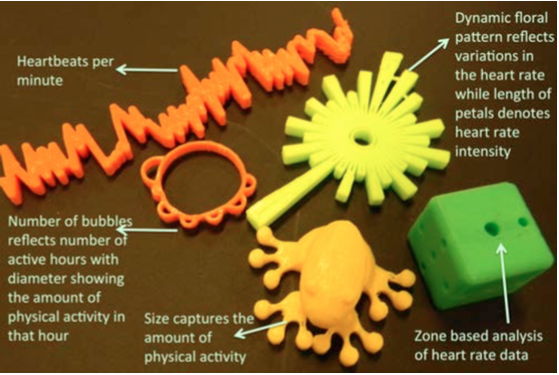
\includegraphics[width=0.7\textwidth]{RelatedWork/img/sweatatoms-as}
  \caption{SweatAtmos activity sculptures\cite{khot2014understanding}}
\label{fig:sweatatmos-as}
\end{center}
\end{figure}

The authors conducted a two week field study with 7 participants with different demographics and exercise habits. Each participant received a 3D printer, a heart-rate sensor and an iPod touch. Participants were required to wear the hear-rate sensor every day. The sensor was paired via bluetooth to the iPod and automatically loaded the data to the SweatAtoms system when the monitoring stopped. SweatAtoms then generated the 5 sculptures from the data. The models were then send to the authors for STL export. Once converted the participants received the STL via email. Participants then proceeded to print the 5 sculptures with the provided 3D printers at home, a procedure that took around two hours. Users kept a diary reflecting on the sculptures and their activity every day. 

The study showed the participants engaged differently with each sculpture. The favorite sculpture was the frog sculpture. The graph was described by a participant as ``not very exciting as we can see the same on a virtual screen''. On the other hand a very active participant liked to see its graph sculpture as he could see how active he had been. For the flower participants expressed different ideas as they could interact with it. A female participant saw the flower suitable for wearing it as earrings. The utility of the rings was often questioned, and was regarded as the least appealing sculpture of the 5. Some users started grouping and assembling the sculptures to form a bigger sculpture. Some users expressed that the dice made them reflect on their lifestyle by analyzing the time they spent on each heart-rate area. The sculptures were also subject of conversations with work colleagues and friends. Users also stated that the value of their heart-rate had gained more significance as the sculptures provided allowed them to ``touch and feel'' their data, this made the sculptures more valuable to participants than screen based visualization. The uniqueness of the objects was repeatedly mentioned by users to be very appealing and the fact of being able to constantly reflect on their activity motivated them to exercise with more intensity.

The SweatAtoms study is a great example of how through activity sculptures motivated users to reflect more about their activity and made them take action. It is surprising to see how participants did not have any trouble at all with the fabrication of the sculptures at their home. The different technologies integrated seamlessly providing a solid set of tools to visualize and easily construct the sculptures. The metaphors utilized to map the data were varied and showed that visualizations that are useful in virtual space not are not necessarily appealing as objects. On the other hand sculptures that were not extremely abstract but rather communicated the data through a playful metaphor, like the frog, were the ones that users liked the most. Overall the SweatAtoms was a very successful project that produced interesting findings regarding activity sculptures and their influence on users.   

\subsubsection{Mental Fabrications}
NeuroSky MindWave Headset

\begin{figure}[h]
\centering
\begin{minipage}{.45\textwidth}
\centering
  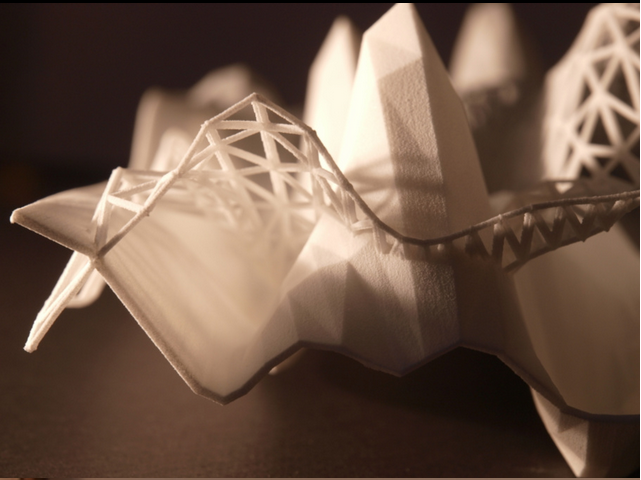
\includegraphics[width=\linewidth]{RelatedWork/img/mentalfab-as}
\end{minipage}
\begin{minipage}{.45\textwidth}
\centering
  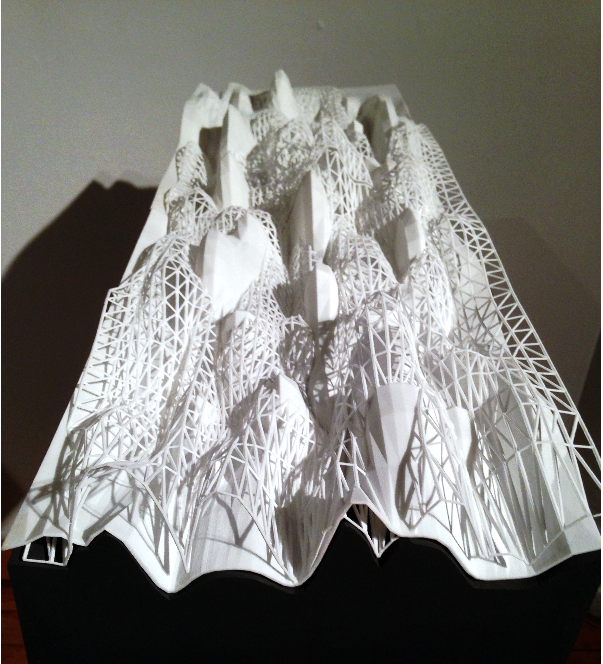
\includegraphics[width=\linewidth,trim= 0mm 37mm 0mm 37mm, clip=true]{RelatedWork/img/mentalfab1-as}
\end{minipage}
\caption{\protect Mental Fabrication's brain activity landscapes\cite{mental2014fabrications}}
\label{fig:mentalfab}
\end{figure}




\subsection{Activity Data Sources}

\subsubsection{Fitness Tracker APIs}

\end{document}